\chapter{Методика распознавания многокомпонентных структур по~разрозненным компонентам (на~примере реидентификации человека)}\label{ch:ch2}

Опираясь на~результаты анализа, представленные в~первой главе, в~данной
главе предлагается комплексная методика распознавания многокомпонентной
структуры по~ее разрозненным связанным компонентам $C_k$ (в~рассматриваемом
случае~--- человек, пара силуэт-лицо, $K=2$), решающая задачу поиска
и~реидентификации в~видеопотоках. Методика включает три
взаимосвязанных компонента: методику детектирования внешнего и~вложенного
компонентов структуры (в~рассматриваемом случае~--- силуэта и~лица),
обеспечивающую корректную локализацию объектов интереса в~различных
сценах и~условиях съемки; методику формирования признаковых представлений
(эмбеддингов) для лицевой и~силуэтной модальностей, ориентированную
на~устойчивую дискриминацию при вариативности ракурса, освещения
и~окклюзий; алгоритм настройки гиперпараметров комбинированной метрики,
обеспечивающий адаптивное взвешивание вклада модальностей и~согласование
качества распознавания с~эксплуатационными ограничениями по~времени
отклика и~ресурсам. Совместное использование указанных компонентов
образует единый контур обработки, в~котором точность последующих этапов
опирается на~качество детектирования, а~итоговое решение формируется
посредством вероятностной интеграции информативных признаков с~учетом
их текущей надежности.

\section{Методика детектирования компонентов структуры (в~рассматриваемом случае~--- силуэтов и~лиц)}\label{sec:ch2/detect}

Методика детектирования компонентов многокомпонентной структуры
(в~рассматриваемом случае~--- силуэтов и~лиц) является ключевым этапом
в~процессе распознавания структуры по~ее разрозненным частям, частным
случаем которого выступает реидентификация человека. Основная задача
на~этом этапе~--- определить и~выделить на~изображениях внешний компонент
структуры (в~рассматриваемом случае~--- силуэт человека). Для этой цели применяются алгоритмы глубокого обучения,
способные обрабатывать и~анализировать сложные визуальные данные.

\subsection{Детектор YOLOv8}\label{sec:ch2/yolov8}

Для задачи обнаружения компонентов структуры (в~рассматриваемом
случае~--- силуэтов и~лиц) в~рамках разработки методики
распознавания многокомпонентных структур и~ее приложения к~реидентификации
человека был выбран
YOLOv8~\cite{Solawetz2023yolov8,Reis2023yolov8flying}~--- одна из~актуальных моделей детектирования объектов. YOLOv8 выделяется способностью
к~быстрому и~точному обнаружению объектов и~поэтому пригодна для задач, требующих обработки вблизи реального времени.
Эта модель, хотя и~не~имеет на~момент написания работы официального
описания, получила широкое распространение в~научном сообществе для решения задач обнаружения объектов. Ее основное преимущество~--- высокие
значения mAP (средняя точность обнаружения) и~низкая задержка обработки
данных, особенно заметная при тестировании на~наборе данных COCO.

Выбор архитектуры YOLOv8 обусловлен сочетанием высокой точности
и~пропускной способности при умеренных вычислительных затратах, что
критично для контура <<детектирование, построение признаковых
представлений, реидентификация>> в~условиях реального времени.
Современные реализации следят за~устойчивостью локализации на~сложных
сценах (плотные сцены, частичные окклюзии, вариативное освещение)
и~обеспечивают стабильно высокие показатели качества на~классических
наборах задач объектной детекции при доступности облегченных
конфигураций модели, пригодных для практического развертывания. Кроме
того, экосистема Ultralytics предусматривает <<из~коробки>> сопряжение
детектора с~трекерами уровня BoT-SORT/ByteTrack и~включение ReID-модуля
(сопоставление по~внешнему виду) на~этапе ассоциации треков, что упрощает
интеграцию YOLOv8 в~конвейер поиска и~реидентификации человека:
параметры трекера содержат явные пороги по~близости и~<<внешности>>,
а~опция \texttt{with\_reid} активирует использование признаковых
представлений для связывания траекторий через окклюзии и~пропуски.
Это делает связку детектора YOLOv8 с~трекером, использующим ReID, распространенным решением для прикладных систем видеоаналитики.

Эффективность такого контура подтверждается прикладными
и~исследовательскими разработками, в~которых YOLOv8 используется как
детектор в~системах отслеживания и~реидентификации: публичные
конвейеры демонстрируют объединение детектора YOLOv8, трекера
Deep/BoT-SORT и~классификационной головы OSNet (ReID) с~устойчивым
сопровождением идентификаторов через временные пропуски и~взаимные
перекрытия объектов; в~ряде проектов дополнительно задействуются
лицевые веса и~позная конфигурация YOLOv8 для повышения надежности
на~человеческих целях. Эти решения иллюстрируют практическую
применимость выбранной архитектуры в~контексте реидентификации
многокомпонентной структуры по~ее частям (в~рассматриваемом случае~---
человека) как завершающего этапа информационно-поискового контура.

Публикации по~BoT-SORT показывают, что включение ReID-признаков
на~этапе ассоциации треков повышает метрики IDF1/HOTA
на~классических бенчмарках MOTChallenge, что опосредованно
подтверждает корректность выбора связки <<точный детектор в~сочетании с~моделью внешнего вида>>.
При использовании в~роли детектора YOLO-семейства (включая YOLOv8)
такой конвейер обеспечивает баланс между качеством и~скоростью,
необходимый для эксплуатации.

В~совокупности эти факторы обосновывают применение YOLOv8 как базовой
архитектуры детектирования в~заявленной методике: модель дает
качественные входные данные для построения эмбеддингов, органично
встраивается в~контур сопровождения и~реидентификации и~обеспечивает требуемые
показатели точности/задержки при реальной нагрузке.

YOLOv8 как модель обнаружения объектов адаптирована для выполнения задач детектирования силуэтов и~лиц.
Основным отличием от~предшественников является улучшенная способность
к~обучению на~разнообразных данных, обеспечивающая выявление более
абстрактных и~сложных визуальных закономерностей. Это достигается за~счет
обучения на~большом и~многообразном наборе данных, включающем
различные категории объектов. Такой подход обеспечивает лучшую
адаптацию модели к~реальным условиям и~различным сценариям
распознавания структур, и~особенно важна при идентификации компонентов
структуры (в~рассматриваемом случае~--- силуэтов и~лиц)
в~сложных и~динамичных условиях.

\begin{figure}[htbp]
\centering
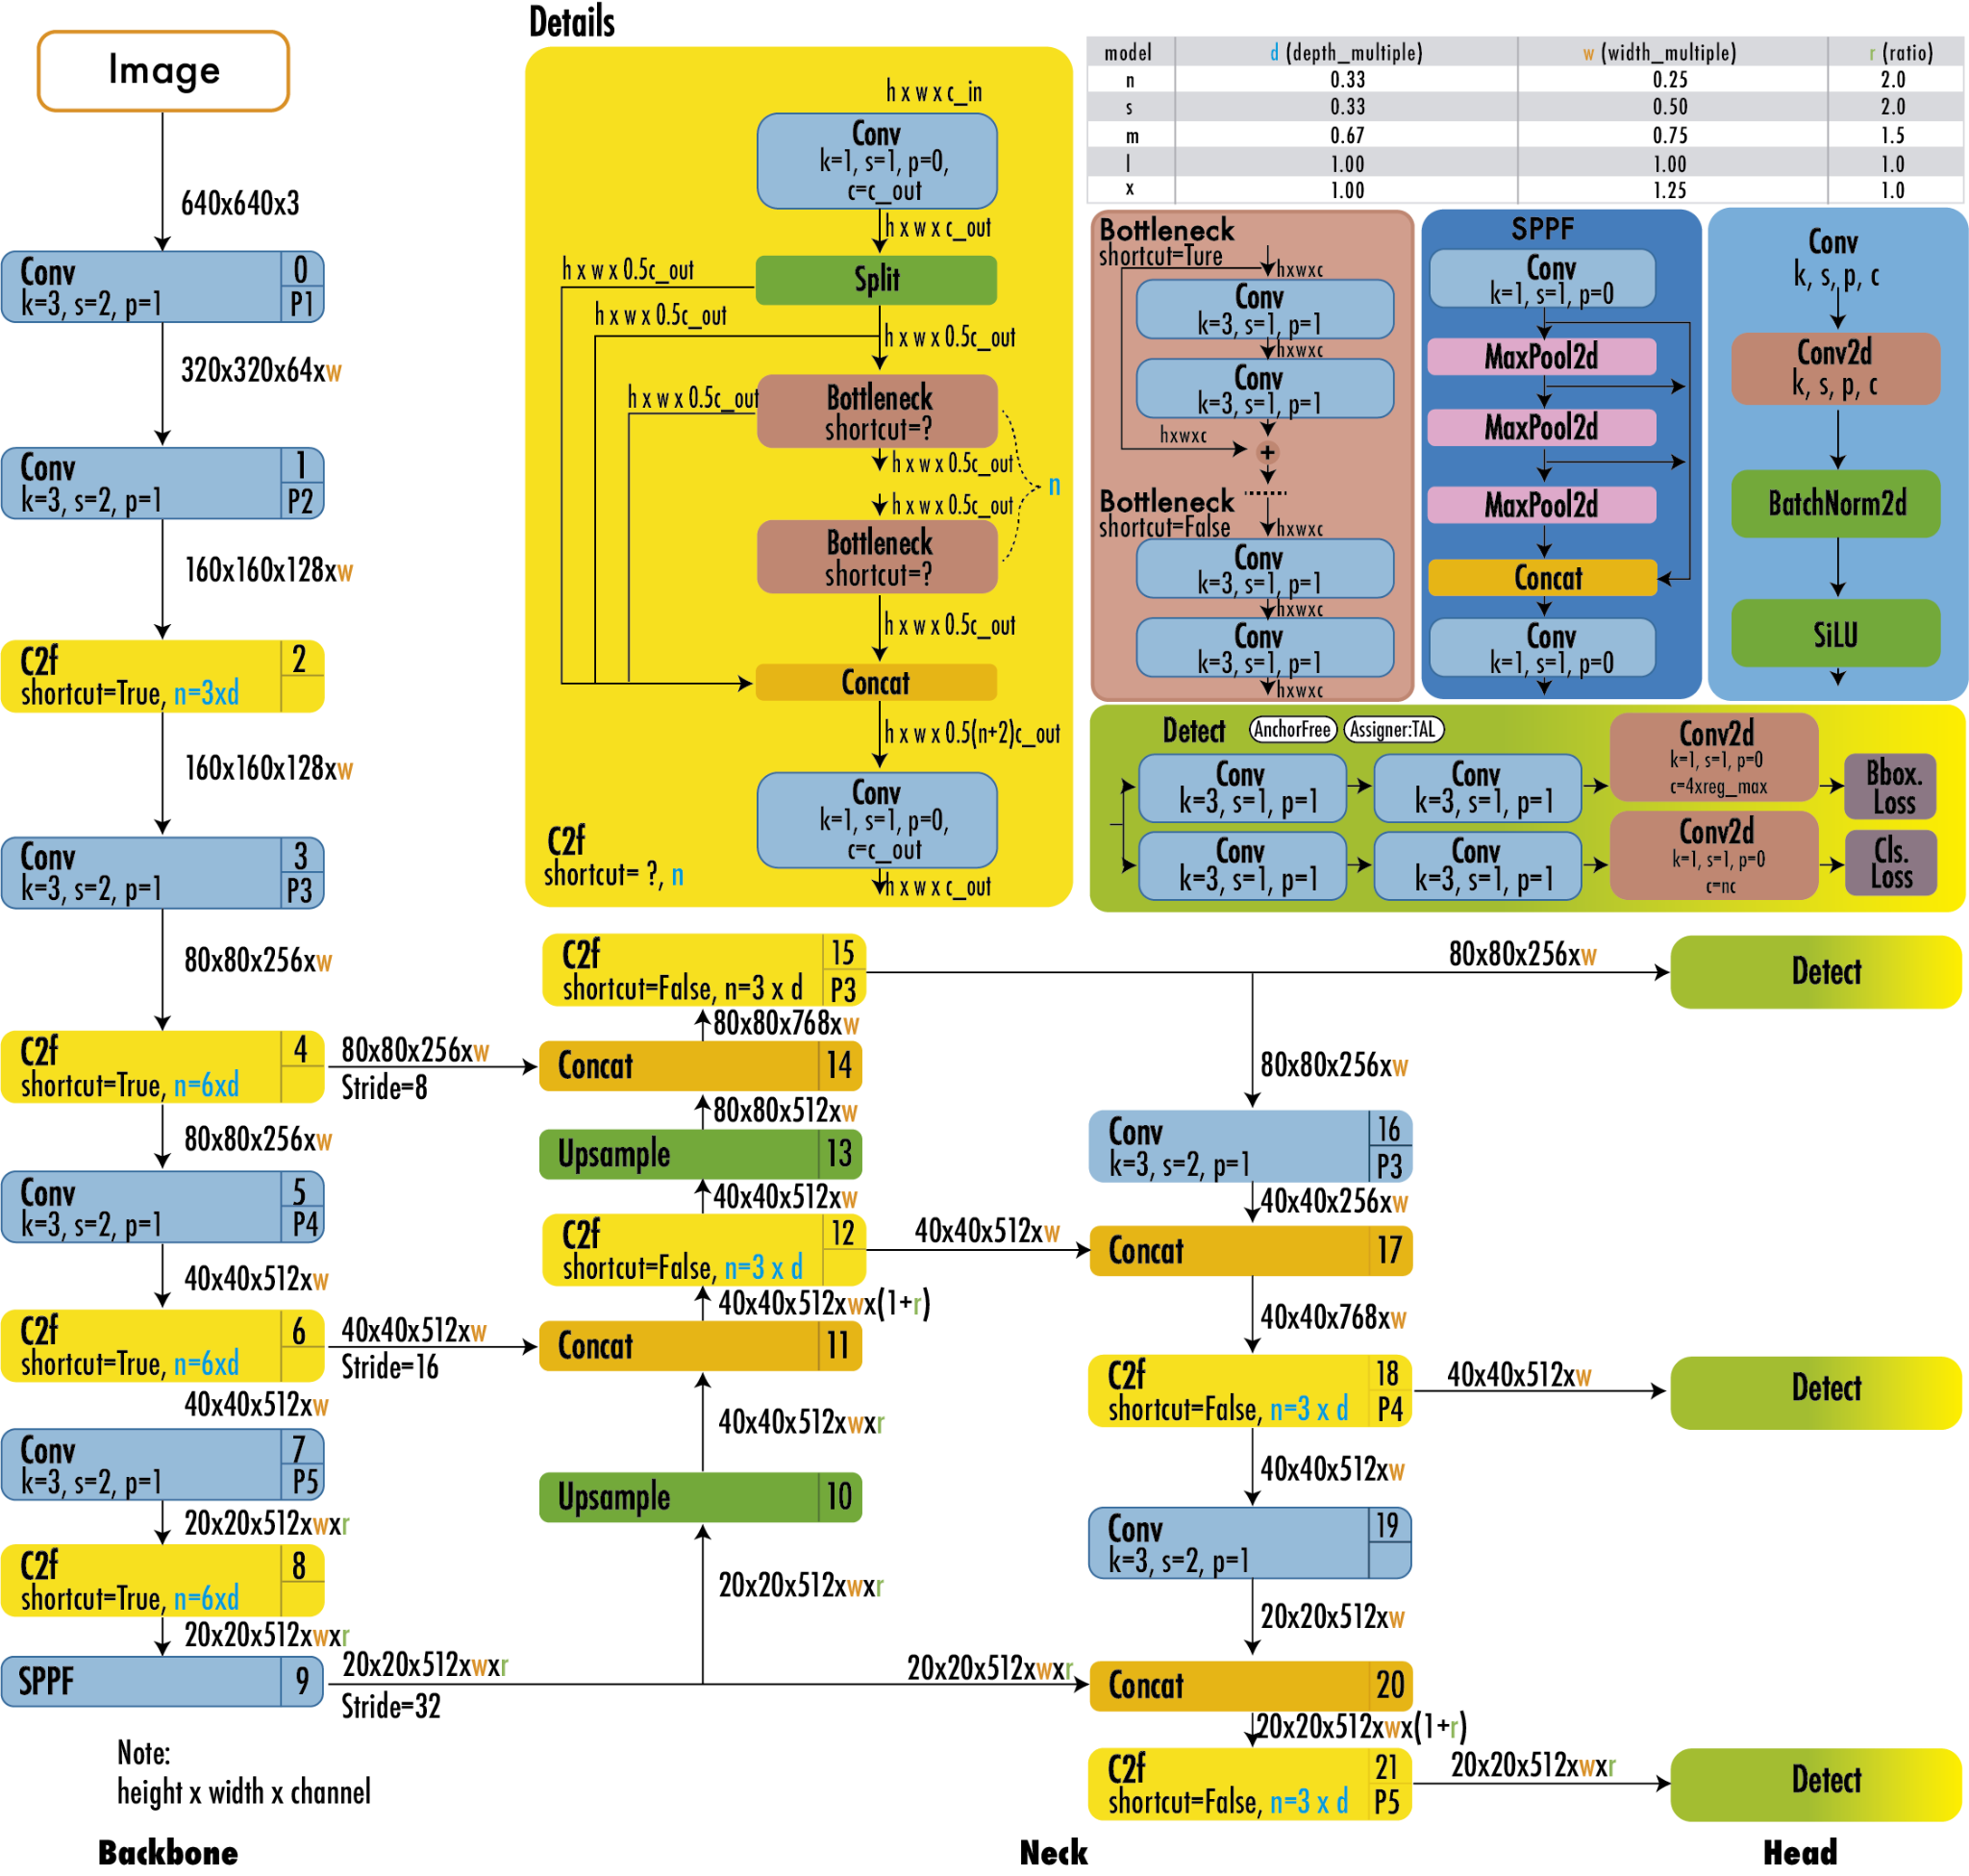
\includegraphics[width=0.85\textwidth,keepaspectratio]{images/2.png}
\caption{Схема архитектуры YOLOv8}
\label{fig:ch2/yolov8}
\end{figure}

На~рис.~\ref{fig:ch2/yolov8} представлена детальная архитектура
YOLOv8. Эта модель развивает концепцию, заложенную в~YOLOv5,
но~с~некоторыми модификациями, в~частности в~модуле CSPLayer, теперь
именуемом как модуль C2f. Модуль C2f (cross-stage partial bottleneck
с~двумя сверточными слоями) объединяет высокоуровневые особенности
с~контекстуальной информацией, что способствует повышению точности
детектирования. YOLOv8 представляет собой модель без якорей
(anchor-free) с~отдельными блоками обработки для определения наличия
объекта, классификации и~регрессии. Такой дизайн обеспечивает
специализацию каждой ветви на~своей задаче, улучшая общую точность
модели. В~выходном слое YOLOv8 используется сигмоидная функция
активации для оценки вероятности наличия объекта в~ограничивающей
рамке. Для оценки вероятностей принадлежности объектов к~классам
применяется покомпонентная сигмоида (бинарная кросс-энтропия).

YOLOv8 использует функции потерь CIoU и~DFL для определения потерь
ограничивающей рамки и~бинарную кросс-энтропию для классификации.
Эти функции потерь обеспечивают улучшенную производительность
детектирования, особенно при работе с~мелкими объектами. Кроме того,
YOLOv8 предлагает модель семантической сегментации, YOLOv8-Seg.
В~ней в~качестве основы используется базовая сеть на~основе CSP-блоков
(CSPDarknet), дополненная модулем C2f вместо традиционной
архитектуры <<шеи>> YOLO. За~модулем C2f расположены две головы
сегментации, обученные предсказывать маски семантической сегментации
для входного изображения. YOLOv8-Seg обеспечивает конкурентоспособные
результаты на~различных бенчмарках по~детектированию объектов
и~семантической сегментации, сохраняя при этом высокую скорость
и~эффективность.

Обобщенная функция потерь и~процедура обновления весов записываются
следующим образом. Уравнение для определения скорости обучения:
\begin{equation}\label{eq:ch2/lr}
    \eta_t=\eta_0\,\gamma^{t},
\end{equation}
где $\eta_0$~--- начальная скорость обучения, $\gamma\in(0,1]$~---
коэффициент затухания, $t$~--- номер итерации.

Правило обновления весов:
\begin{equation}\label{eq:ch2/sgd}
    \theta_{t+1}=\theta_t-\eta_t\,\nabla_\theta\mathcal{L}(\theta_t),
\end{equation}
где $\theta$~--- параметры модели, $\mathcal{L}$~--- функция потерь.

Конкретная функция потерь YOLOv8 определяется следующим образом:
\begin{equation}\label{eq:ch2/yolo-loss}
    \mathcal{L}_{\text{YOLO}}=\lambda_{\text{box}}\,\mathcal{L}_{\text{CIoU}}+\lambda_{\text{cls}}\,\mathcal{L}_{\text{BCE}}+\lambda_{\text{dfl}}\,\mathcal{L}_{\text{DFL}},
\end{equation}
где $\mathcal{L}_{\text{CIoU}}$~--- потери на~ограничивающей рамке,
$\mathcal{L}_{\text{BCE}}$~--- бинарная кросс-энтропия для
поклассовой классификации (в~режиме <<один против остальных>>), $\mathcal{L}_{\text{DFL}}$~---
distribution focal loss; $\lambda_{\text{box}},\lambda_{\text{cls}},\lambda_{\text{dfl}}$~---
весовые коэффициенты компонентов.

Потери CIoU вычисляются как:
\begin{equation}\label{eq:ch2/ciou}
    \mathcal{L}_{\text{CIoU}}=\frac{1}{N_{\text{pred}}}\sum_{i=1}^{N_{\text{pred}}}\mathbb{I}_{\text{obj}}(i)\bigl[1-\mathrm{IoU}(\hat{B}_i,B_i)+\frac{\rho^2(\hat{c}_i,c_i)}{d_i^2}+\alpha\,v_i\bigr],
\end{equation}
где $N_{\text{pred}}$~--- общее количество ячеек, содержащих объект;
$\mathbb{I}_{\text{obj}}(i)$~--- индикаторная функция для ячеек,
содержащих объект; $\hat{B}_i$~--- предсказанная ограничивающая рамка;
$B_i$~--- истинная ограничивающая рамка; $\hat{c}_i,c_i$~--- центры
рамок; $\rho^2$~--- квадрат евклидова расстояния; $d_i$~--- диагональ
наименьшей охватывающей рамки; $\alpha,v_i$~--- коэффициенты учета
соотношения сторон.

Эта функция потерь включает в~себя потери CIoU для точности
ограничивающей рамки, стандартную двоичную кросс-энтропию (поклассово,
в~режиме <<один против остальных>>) и~распределенные фокальные потери (distribution focal loss).

Протестированный на~наборе данных MS~COCO test-dev~2017, YOLOv8x
показал точность AP~53,9\% при размере изображения 640~пикселей,
превосходя по~этому показателю предшествующие версии семейства YOLO, при этом
скорость составила 280~кадров в~секунду на~NVIDIA~A100 и~TensorRT.

\subsection{Функции потерь для совместного детектирования внешнего и~вложенного компонентов структуры (в~рассматриваемом случае~--- силуэтов и~лиц людей)}\label{sec:ch2/loss}

В~рамках улучшения методики распознавания многокомпонентной структуры
по~ее разрозненным частям, частным случаем которой является реидентификация
человека, была разработана новая функция потерь, направленная на~более точное
детектирование вложенного компонента внутри внешнего (в~рассматриваемом
случае~--- лица внутри силуэта). Эта модификация функции потерь
учитывает не~только общие характеристики объекта, но~и~специфику
расположения вложенного компонента в~пределах внешнего (лица в~пределах силуэта). Разработка усовершенствованной
функции потерь для детектирования вложенного компонента внутри внешнего
(в~рассматриваемом случае~--- лиц в~силуэтах) включает в~себя
интеграцию нового компонента в~стандартную функцию потерь модели
YOLOv8. Формула новой функции потерь имеет вид:
\begin{equation}\label{eq:ch2/loss-modified}
    \mathcal{L}=\mathcal{L}_0+\lambda_{\text{inner}}\,\frac{1}{N_{\text{pred}}}\sum_{i=1}^{N_{\text{pred}}}\mathbb{I}_{\text{inner}}(i)\,\mathcal{L}_{\text{inner}}(i),
\end{equation}
где $\mathcal{L}_0$ обозначает исходную функцию потерь YOLOv8;
$\lambda_{\text{inner}}$~--- коэффициент, задающий вес нового компонента
в~общей функции потерь; $N_{\text{pred}}$~--- общее количество ячеек
с~объектами; $\mathbb{I}_{\text{inner}}(i)$~--- индикаторная функция,
определяющая, содержит ли $i$-я ячейка лицо; $\mathcal{L}_{\text{inner}}(i)$~---
компонент функции потерь для детекции лица внутри ограничивающей рамки
силуэта.

Основной принцип работы новой функции потерь заключается в~повышении
точности идентификации вложенного компонента структуры (в~рассматриваемом
случае~--- лица) в~сложных сценариях. Это достигается
за~счет штрафования модели в~случаях неправильного обнаружения вложенного
компонента внутри внешнего (лица внутри силуэта) или его отсутствия, когда
оно ожидалось. Таким образом,
модель становится более чувствительной к~положению вложенного компонента
в~рамках внешнего (в~рассматриваемом случае~--- лица в~рамках силуэта),
и~повышает общую точность системы распознавания структуры по~ее частям. Новая
функция потерь разработана на~основе понимания динамических условий
визуального распознавания лиц. Она учитывает ряд критически важных
факторов: частичное закрытие лица, нестандартные углы наблюдения
и~переменную освещенность. Теоретически такой подход повышает
чувствительность модели к~мелким деталям и~улучшает ее способность
к~распознаванию лиц в~менее очевидных или прямых сценариях.

Внедрение новой функции потерь обеспечивает улучшение общей
производительности системы в~следующих аспектах:
\begin{itemize}
    \item основное предназначение новой функции потерь~--- улучшение
          точности идентификации лиц в~условиях, где традиционные
          модели могут испытывать затруднения (например, при частично
          закрытом лице);
    \item в~условиях быстрого изменения сцен (например, в~местах
          массового скопления людей), где лица могут появляться
          и~исчезать в~кадре, новая функция потерь помогает модели
          быстрее адаптироваться к~изменениям и~эффективнее
          идентифицировать лица;
    \item путем штрафования за~ошибки детектирования вложенного компонента вне
          границ внешнего (в~рассматриваемом случае~--- вне силуэтов) или
          пропуски вложенного компонента, когда он должен быть обнаружен,
          функция
          потерь способствует снижению ложных положительных
          и~отрицательных срабатываний.
\end{itemize}

\section{Байесовская модель объединения признаковых представлений компонентов структуры (в~задаче реидентификации личности как частном случае)}\label{sec:ch2/bayes}

В~отличие от~традиционных подходов, опирающихся на~один биометрический
фактор, разработана универсальная методика объединения признаков,
полученных из~разных источников информации. В~основе метода лежит
вероятностная модель, реализующая объединение признаков в~пространстве
решений по~правилу байесовского вывода. Каждый признак рассматривается
как наблюдение, аппроксимируемое нормальным распределением
с~параметрами, оцениваемыми по~обучающим данным. Принятие решения
осуществляется путем максимизации апостериорной вероятности
принадлежности объекта к~одной из~известных личностей. В~качестве
средств извлечения признаков используются модели на~основе архитектур
с~механизмами внимания, обеспечивающие устойчивость к~искажениям.
Проведено сравнение с~методом линейного объединения признаков.
Результаты экспериментов на~открытом наборе данных демонстрируют
повышение точности идентификации, устойчивость к~частичному отсутствию
данных и~возможность количественной оценки степени достоверности
принимаемого решения, что актуально для применения в~системах
обеспечения безопасности.

В~общей постановке рассматривается распознавание многокомпонентной
структуры по~ее разрозненным частям~--- связанным компонентам $C_k$,
извлекаемым из~разных источников информации. В~рассматриваемом случае
такой структурой выступает человек, а~ее компонентами~--- пара
<<силуэт-лицо>> ($K=2$), и~соответствующая прикладная задача~---
реидентификация человека (ReID)~--- состоит
в~поиске и~распознавании одного и~того же человека на~различных снимках
или в~разных камерах наблюдения~\cite{Khachumov2015face}. Актуальность
ReID обусловлена активным развитием систем видеонаблюдения и~вопросами
безопасности: автоматическое отслеживание перемещений подозреваемых,
поиск пропавших людей и~т.\,п.~\cite{Vezzani2013reidsurvey}.

Традиционно ReID опирается либо на~биометрию лица, либо на~общие
признаки фигуры (силуэт, одежда) человека по~отдельности. Однако,
только на~одном источнике (лицо или тело) достичь высокой надежности
распознавания сложно из-за вариаций позы, освещения, разрешения
и~перекрытий. Совмещение нескольких биометрических признаков повышает
точность за~счет взаимодополняющей информации различных
модальностей~\cite{Irfan2022multimodal,Koo2018multimodal}.

В~частности, силуэт человека считается почти таким же уникальным, как
и~лицо, и~уже используется на~практике. Так, новейшие отечественные
системы умного видеонаблюдения отслеживают траекторию по~силуэтам
и~осуществляют поиск по~фигуре в~реальном
времени~\cite{Telenkov2021silhouette}. Вместе с~тем возникает вопрос
эффективной интеграции разнородных признаков.

Наиболее простой подход объединения признаков компонентов структуры~---
линейная комбинация,
например, конкатенация векторов компонентов (в~рассматриваемом
случае~--- лица и~тела) или усреднение оценок
совпадения~\cite{Koo2018multimodal}. Однако жесткое фиксированное
слияние имеет ряд ограничений. Во-первых, оно не~учитывает надежность
каждой модальности: <<шумные>> данные (например, размытое лицо или
скрытая одежда) могут снижать итоговую точность, тогда как оптимально
было бы придать им меньший вес. Во-вторых, линейное слияние не~отражает
вероятностную природу биометрических измерений и~не~дает информации
о~степени уверенности. В~результате система может ошибаться в~условиях
искаженного входа, не~имея механизма выражения неуверенности
в~принятом решении.

В~данной работе впервые предлагается использовать вероятностную модель
на~основе теоремы Байеса для объединения представлений отдельных
компонентов многокомпонентной структуры (в~рассматриваемом случае~---
многомодальных представлений лица и~тела человека). Научная новизна
заключается в~том, что байесовский подход
обеспечивает адаптивное взвешивание вклада каждого компонента через
его правдоподобие (остроту гауссова распределения класса), повышая
устойчивость системы к~шуму,
изменению условий съемки и~отсутствию одного из~компонентов структуры
(в~частном случае~--- одного из~биометрических факторов).

В~работе представлены:
\begin{enumerate}[label=\alph*)]
    \item формальная модель и~алгоритм байесовской интеграции
          признаков;
    \item ее программная реализация с~использованием современных
          нейросетевых архитектур (Vision Transformer) и~функции потерь
          ArcFace;
    \item экспериментальное сравнение с~традиционным линейным подходом
          на~открытом наборе данных.
\end{enumerate}

\subsection{Распознавание по~отдельным компонентам структуры (лицо и~тело)}\label{sec:ch2/face-body}

Исторически распознавание отдельных компонентов структуры развивалось
независимо: применительно к~рассматриваемому случаю задача
распознавания лица по~изображениям длительное время развивалась
независимо от~задачи ReID по~силуэту, формируя собственные подходы
и~методы. С~появлением глубоких нейросетей были достигнуты высокие
результаты: так, архитектура FaceNet с~триплетным
обучением~\cite{Schroff2015facenet} достигла точности 99,6\%
на~эталонном наборе данных LFW.

В~дальнейшем были предложены специальные функции потерь, направленные
на~повышение дискриминативности векторов лица. Одной из~наиболее
эффективных стала функция ArcFace~\cite{Deng2019arcface}, которая
вводит аддитивную угловую поправку-отступ в~классификационное обучение,
обеспечивая более плотные кластеры векторов для каждого человека.
В~настоящее время ArcFace широко применяется в~задачах распознавания
лиц; его эффективность подтверждена как зарубежными, так
и~отечественными исследованиями~\cite{Mubinova2024face}.

Тем не~менее даже лучшие модели распознавания лиц могут давать сбои
в~условиях неконтролируемой съемки~--- при низком разрешении,
поворотах головы, частичном закрытии лица (маски,
шарфы)~\cite{Mubinova2024face}. В~частности, отечественные работы
отмечают снижение качества на~<<нетипичных>> лицах, существенно
отличающихся от~доминирующих в~обучающих данных (например, лица детей
или представителей редких рас)~\cite{Sokolova2022face}, и~предлагают
методы предварительной фильтрации <<сложных>> случаев для повышения
надежности. Одновременно со~стороны ReID по~фигуре также наблюдается
значительный прогресс. Классические подходы опирались на~признаки
внешнего вида: цветовые гистограммы, HOG-описатели, локальные
инвариантные признаки и~другие~\cite{Khachumov2015face}. С~развитием
глубокого обучения акцент сместился на~обучаемые вектора изображений
полноростового человека~\cite{Vezzani2013reidsurvey}.

Архитектуры на~основе сверточных нейронных сетей (например, ResNet-50)
обучаются либо классифицировать личности в~тренировочном наборе
с~использованием функции Softmax, либо непосредственно оптимизировать
вектора с~помощью метрического обучения (триплетная и~контрастивная
функции потерь и~т.\,п.)~\cite{Hermans2017triplet}. Для повышения устойчивости
к~вариациям позы используются стратегии деления тела на~части
и~механизмы внимания.

Так, Harmonious Attention Network (HAN) объединяет пространственное
и~каналовое внимание для выделения наиболее информативных областей
изображения человека~\cite{LiW2018harmonious}. Другие работы
задействуют скелетную позу как условие для объединения признаков или
применяют графовые нейронные сети (Graph Convolutional Networks, GCN)
для моделирования взаимосвязей между частями тела и~визуальными
атрибутами~\cite{Liao2023mmmgcn}.

В~целом современные модели реидентификации человека демонстрируют
высокое качество на~стандартных бенчмарках (Market-1501, MSMT17 и~др.),
особенно при использовании нескольких масштабов и~агрегации локальных
признаков частей тела~\cite{Ignatyeva2024reid}. Тем не~менее
большинство существующих решений опираются исключительно на~один
компонент структуры~--- в~рассматриваемом случае на~единственную
визуальную модальность, внешний вид человека.

\subsection{Интеграция многомодальных биометрических признаков}\label{sec:ch2/multimodal}

Комбинация признаков нескольких компонентов структуры (в~рассматриваемом
случае~--- лица и~полного силуэта человека) представляет собой
мультибиометрический подход к~идентификации. Еще в~ранних работах
отмечалось, что объединение нескольких биометрических идентификаторов
(например, лица, радужной оболочки, голоса) повышает общую точность
системы за~счет разнородности используемых источников.

В~задаче ReID предпринимались различные подходы к~многомодальной
интеграции признаков на~разных уровнях. Простейший из~них~--- объединение на~уровне
признаков: например, конкатенация векторов лица и~тела с~последующей
классификацией или вычислением
расстояний~\cite{Koo2018multimodal}. Такой метод использован
в~работе~\cite{Shoukry2022multimodal}, где отдельные нейросети
извлекают признаки лица (FaceNet) и~тела (OSNet), после чего векторы
объединяются и~сравниваются с~эталонными комбинациями; авторы
демонстрируют прирост порядка~5\% в~метрике Rank-1 по~сравнению
с~использованием только тела.

Более сложные схемы реализуют слияние на~уровне оценок, например посредством усреднения или обучаемого взвешивания
сходства между лицом и~фигурой~\cite{Koo2018multimodal}. В~системах
высокого уровня применяются также байесовские сети доверия, где выходы
детектора лица и~дополнительная информация (пол, возраст, рост)
интегрируются для повышения надежности идентификации
в~робототехнических приложениях~\cite{Khachumov2015face}.

Важным направлением является применение механизмов перекрестного
внимания между модальностями, обеспечивающих самостоятельное выявление
моделью того, каким признакам следует уделять больше внимания.
В~недавней работе~\cite{Vezzani2013reidsurvey}, объединяющей визуальные
и~языковые описания, демонстрируется улучшение ReID за~счет
одновременного использования лица и~тела: на~основе изображения
генерируется текстовое описание, и~модули внимания сопоставляют текст
с~соответствующими областями (лицо, тело) на~изображении, обеспечивая
более полную идентификацию.

Графовые подходы, в~частности основанные на~GCN, представляют
мультимодальные признаки в~виде графа, где узлы соответствуют векторам
разных модальностей одного человека, а~ребра отражают их
принадлежность к~одной личности~\cite{Zhong2020personsearch}. Обучение
такого графа обеспечивает эффективное распространение информации между
модальностями.

В~большинстве рассмотренных подходов (за~исключением байесовских)
интеграция осуществляется либо через обучаемые веса, неявно
аппроксимирующие байесовский вывод, либо через механизмы
внимания. Однако явная вероятностная интеграция по~правилу Байеса
до~сих пор не~применялась для слияния векторов отдельных компонентов
структуры (в~рассматриваемом случае~--- лица и~тела человека). Между тем
в~смежных областях байесовские методы доказали свою эффективность при
принятии решений на~основе нескольких источников
информации~\cite{Koo2018multimodal}. В~данной работе восполняется этот
пробел путем предложения явной байесовской модели для объединения
векторов компонентов структуры (в~рассматриваемом случае~--- в~задаче ReID).

Таким образом, предложенный подход концептуально близок
к~мультибиометрическим системам, осуществляющим объединение признаков
на~уровне принятия решения. Однако в~отличие от~существующих решений
он основан не~на~эвристических или обучаемых весах, а~на~строгом
байесовском выводе.

Разработанная схема может быть интерпретирована как наивный
байесовский классификатор класса структуры (в~рассматриваемом
случае~--- личности человека), в~котором признаками выступают
векторы компонентов структуры (в~частном случае~--- лица и~силуэта). Ранее наивный Байес использовался
в~биометрических системах для принятия решений по~отпечаткам пальцев
и~изображениям лиц~\cite{Koo2018multimodal}, но~не~в~контексте
глубоких нейросетевых векторов.

В~работе применяются современные
высокоуровневые подходы~--- ArcFace и~Vision Transformer,
обеспечивающие компактное и~устойчивое представление каждой
модальности. Это принципиально отличает предложенный метод от~более
ранних работ, основанных на~низкоуровневых визуальных
признаках~\cite{Khachumov2015face}.

\subsection{Байесовская модель интеграции}\label{sec:ch2/bayes-model}

\paragraph{Общий случай: произвольное число компонентов структуры.}
В~общей постановке наблюдаемый объект представляет собой
многокомпонентную структуру, описываемую конечным множеством
независимо извлекаемых признаковых описаний
$\{\mathbf{z}_k\colon k=1,\ldots,K\}$, где $K\ge 2$~--- число
компонентов структуры, а~$\mathbf{z}_k\in\mathbb{R}^{d_k}$~---
эмбеддинг, формируемый кодировщиком~$\Phi_k$ по~$k$-му компоненту.
В~эксплуатационных режимах ИПС не~все компоненты доступны
одновременно: множество наблюдаемых в~момент~$t$ компонентов
$\mathcal{M}(t)\subseteq\{1,\ldots,K\}$ является случайной величиной,
определяемой условиями съемки (окклюзии, ракурс, разрешение).

Задача распознавания структуры формулируется как многоклассовая
вероятностная классификация: по~доступным эмбеддингам
$\{\mathbf{z}_k\colon k\in\mathcal{M}(t)\}$ требуется найти
оценку класса
\begin{equation}\label{eq:ch2/bayes-generic}
    y^{*}=\arg\max_{y\in Y}P\!\left(y\mid\{\mathbf{z}_k\colon k\in\mathcal{M}(t)\}\right).
\end{equation}
При допущении условной независимости компонентов структуры
относительно~$y$ апостериорная вероятность факторизуется
по~правилу Байеса:
\begin{equation}\label{eq:ch2/bayes-factor-generic}
    P\!\left(y\mid\{\mathbf{z}_k\}\right)\propto P(y)\prod_{k\in\mathcal{M}(t)}P(\mathbf{z}_k\mid y),
\end{equation}
а~при равноправных классах ($P(y)=\mathrm{const}$) решающее
правило сводится к~многоклассовому MAP-критерию:
\begin{equation}\label{eq:ch2/map-generic}
    y^{*}=\arg\max_{y\in Y}\sum_{k\in\mathcal{M}(t)}\log P(\mathbf{z}_k\mid y).
\end{equation}
Аппроксимация модально-зависимых правдоподобий
$P(\mathbf{z}_k\mid y)$ многомерным нормальным распределением
\begin{equation}\label{eq:ch2/gauss-generic}
    P(\mathbf{z}_k\mid y)=
    \frac{1}{(2\pi)^{d_k/2}|\Sigma_{y,k}|^{1/2}}
    \exp\!\left(-\tfrac{1}{2}(\mathbf{z}_k-\boldsymbol{\mu}_{y,k})^{T}\Sigma_{y,k}^{-1}(\mathbf{z}_k-\boldsymbol{\mu}_{y,k})\right)
\end{equation}
обеспечивает автоматическое взвешивание компонентов через
ковариационные матрицы класса $\Sigma_{y,k}$: чем компактнее
внутриклассовый кластер компонента~$k$ в~признаковом пространстве,
тем <<острее>> правдоподобие и~тем сильнее вклад этого компонента
в~argmax. Тем самым адаптивный учет надежности достигается без
ручной подстройки весов и~без введения дополнительного гиперпараметра
комбинирования. При отсутствии $k$-го компонента
($k\notin\mathcal{M}(t)$) соответствующее слагаемое исключается
из~(\ref{eq:ch2/map-generic}), что эквивалентно маргинализации
по~отсутствующему наблюдению и~обеспечивает корректное поведение
решающего правила в~условиях неполноты данных.

\paragraph{Частный случай: $K=2$, реидентификация людей по~паре <<силуэт-лицо>>.}
В~настоящей работе общая постановка
(\ref{eq:ch2/bayes-generic})--(\ref{eq:ch2/gauss-generic})
экспериментально проверяется на~наиболее представительной задаче
с~$K=2$: компонентами структуры выступают лицо и~силуэт человека,
а~их признаковые описания обозначаются $\mathbf{z}_1\equiv\mathbf{f}$
(лицо) и~$\mathbf{z}_2\equiv\mathbf{s}$ (силуэт). С~учетом этого
выражения~(\ref{eq:ch2/bayes-generic})--(\ref{eq:ch2/map-generic})
конкретизируются следующим образом.

В~рассматриваемом частном случае $K=2$ задача распознавания структуры
моделируется как статистическая классификация
класса~$y$ (личности человека) по~двум наблюдениям~--- наблюдаемым
компонентам структуры: вектору признаков лица~$\mathbf{f}$
и~вектору признаков силуэта~$\mathbf{s}$. Пусть $y$~--- дискретная
случайная переменная, принимающая значения из~множества классов
идентификации~$Y$ (известных системе личностей). Тогда по~теореме
Байеса апостериорная вероятность того, что наблюдения
$(\mathbf{f},\mathbf{s})$ принадлежат человеку~$y$, определяется как:
\begin{equation}\label{eq:ch2/bayes}
    P(y\mid\mathbf{f},\mathbf{s})=\frac{P(\mathbf{f}\mid y)\,P(\mathbf{s}\mid y)\,P(y)}{\sum\limits_{y'\in Y}P(\mathbf{f}\mid y')\,P(\mathbf{s}\mid y')\,P(y')},
\end{equation}
где $P(\mathbf{f}\mid y)$~--- правдоподобие наблюдаемого признака лица
при условии личности~$y$; $P(\mathbf{s}\mid y)$~--- правдоподобие
признака силуэта; $P(y)$~--- априорная вероятность личности~$y$.
В~настоящей работе априорно все кандидаты равновероятны
(непредвзятая идентификация), поэтому далее полагается
$P(y)=\mathrm{const}$. Таким образом, решение о~том, что
на~изображении представлен человек~$y^*$, принимается по~правилу
максимума апостериорной вероятности (MAP):
\begin{equation}\label{eq:ch2/map}
    y^*=\arg\max_{y\in Y}\bigl[\log P(\mathbf{f}\mid y)+\log P(\mathbf{s}\mid y)\bigr],
\end{equation}
где переход к~логарифмическим правдоподобиям заменяет произведение
плотностей на~сумму логарифмов и~предотвращает переполнение при работе
с~малыми величинами вероятностей, а~также обеспечивает численную
устойчивость вычислений. Выражение~(\ref{eq:ch2/map}) показывает, что
решение складывается из~двух логарифмических правдоподобий~---
от~лица и~от~силуэта. Если, например, лицо плохо распозналось (низкое
$P(\mathbf{f}\mid y)$), но~силуэт совпал уверенно (высокое
$P(\mathbf{s}\mid y)$), то~личность все равно может быть правильно
определена за~счет второй части. И~наоборот, при противоречивых
признаках будет выбран тот кандидат~$y$, для которого произведение
плотностей (или сумма логарифмов) максимизируется~--- то~есть оба
признака достаточно соответствуют этому кандидату лучше, чем любому
другому. Такая схема эквивалентна наивному байесовскому
классификатору, учитывающему независимые <<признаковые условия>>
$\mathbf{f}$ и~$\mathbf{s}$ для каждого класса~$y$~\cite{Koo2018multimodal}.
В~настоящем случае условная независимость признаков лица и~тела~---
упрощающее предположение (наивный Байес), оправданное раздельным
обучением кодировщиков и~различной природой модальностей.

Для вычисления $P(\mathbf{f}\mid y)$ и~$P(\mathbf{s}\mid y)$ необходимо
построить вероятностную модель распределения векторов каждой
модальности для каждой личности. В~данном исследовании выбирается
простейшая модель~--- многомерное нормальное распределение
(гауссиана) в~пространстве векторов. Предполагается, что для каждой
личности~$y$ признаки лица $\mathbf{f}$ распределены нормально
с~некоторым средним $\boldsymbol{\mu}_y^f$ и~ковариационной матрицей
$\Sigma_y^f$, то~же верно для признаков силуэта с~параметрами
$\boldsymbol{\mu}_y^s,\Sigma_y^s$. Эти параметры можно оценить
по~обучающей выборке векторов (то~есть по~нескольким изображениям
каждого человека из~базы). Тогда плотность имеет вид:
\begin{equation}\label{eq:ch2/gauss}
    P(\mathbf{f}\mid y)=\frac{1}{(2\pi)^{d/2}\,|\Sigma_y^f|^{1/2}}\exp\!\left(-\tfrac{1}{2}(\mathbf{f}-\boldsymbol{\mu}_y^f)^{T}{\Sigma_y^f}^{-1}(\mathbf{f}-\boldsymbol{\mu}_y^f)\right),
\end{equation}
и~аналогично для $P(\mathbf{s}\mid y)$. Здесь $d$~--- размерность
пространства эмбеддинга соответствующей модальности (для лица $d_f=128$, для силуэта $d_s=256$). На~практике для
устойчивости и~уменьшения числа параметров возможно использование
диагональной или изотропной (скалярной $\sigma^2 I$) ковариации,
тогда формулы упрощаются до~зависимости от~евклидова или
махаланобисова расстояния
$\lVert\mathbf{f}-\boldsymbol{\mu}_y^f\rVert$.

Таким образом, при изотропной ковариации байесовский подход сводится
к~распознаванию по~ближайшему центроиду в~евклидовой метрике, а~при
диагональной или полной ковариации~--- по~махаланобисову (взвешенному
по~дисперсии) расстоянию.
Полноценная же байесовская модель~(\ref{eq:ch2/gauss}) допускает
задание разных ковариаций, учитывая, например, что разброс признаков
лица для данной личности меньше, чем разброс признаков фигуры (поскольку одежда меняется).

Обобщенная блок-схема предлагаемой байесовской интеграции для
произвольного числа компонентов структуры $K$ приведена
на~рис.~\ref{fig:ch2/bayes-generic}: доступные эмбеддинги
$\{\mathbf{z}_k\colon k\in\mathcal{M}(t)\}$ независимо преобразуются
в~логарифмы гауссовых правдоподобий, которые суммируются по~доступным
компонентам, а~максимизация по~$y\in Y$ задает MAP-решение.
Конкретизация этой схемы для рассматриваемого случая $K=2$
(реидентификация по~паре <<силуэт-лицо>>) приведена
на~рис.~\ref{fig:ch2/bayes-scheme}.

\begin{figure}[htbp]
\centering
% Обобщённая блок-схема байесовской интеграции K компонентов
\begin{tikzpicture}[
    node distance=5mm and 6mm,
    every node/.style={font=\small},
    block/.style={
        draw, rounded corners, align=center,
        minimum height=8mm, minimum width=26mm,
        inner sep=2pt
    },
    gauss/.style={
        draw, align=center,
        minimum height=10mm, minimum width=42mm,
        inner sep=2pt, fill=black!3
    },
    arr/.style={-{Latex[length=2mm]}, thick},
    dots/.style={font=\Large},
]
% Вход
\node[block] (input) {Доступные эмбеддинги\\ $\{\mathbf{z}_k\colon k\in\mathcal{M}(t)\}$};

% Гауссовы правдоподобия
\node[gauss, below=8mm of input.south west, anchor=north west] (g1)
    {$\log P(\mathbf{z}_1\mid y)$\\ $=-\tfrac{1}{2}\,d_{\mathrm{M}}^{2}(\mathbf{z}_1;\boldsymbol{\mu}_{y,1},\Sigma_{y,1})+c_1$};
\node[gauss, right=6mm of g1] (g2)
    {$\log P(\mathbf{z}_2\mid y)$\\ $=-\tfrac{1}{2}\,d_{\mathrm{M}}^{2}(\mathbf{z}_2;\boldsymbol{\mu}_{y,2},\Sigma_{y,2})+c_2$};
\node[dots, right=4mm of g2] (gdots) {$\cdots$};
\node[gauss, right=4mm of gdots] (gK)
    {$\log P(\mathbf{z}_K\mid y)$\\ $=-\tfrac{1}{2}\,d_{\mathrm{M}}^{2}(\mathbf{z}_K;\boldsymbol{\mu}_{y,K},\Sigma_{y,K})+c_K$};

\draw[arr] (input.south) -- ++(0,-3mm) -| (g1.north);
\draw[arr] (input.south) -- ++(0,-3mm) -| (g2.north);
\draw[arr] (input.south) -- ++(0,-3mm) -| (gK.north);

% Сумматор
\node[block, below=12mm of g2, minimum width=70mm] (sum)
    {Суммирование лог-правдоподобий по~доступным компонентам\\ $\displaystyle S(y)=\sum_{k\in\mathcal{M}(t)}\log P(\mathbf{z}_k\mid y)$};
\draw[arr] (g1.south) -- (sum.north -| g1);
\draw[arr] (g2.south) -- (sum.north -| g2);
\draw[arr] (gK.south) -- (sum.north -| gK);

% MAP
\node[block, below=5mm of sum, minimum width=70mm]
    (map) {Выбор по~MAP-критерию: $y^{*}=\displaystyle\arg\max_{y\in Y}S(y)$};
\draw[arr] (sum) -- (map);

% Решение и доверие
\node[block, below=5mm of map] (out) {Решение $y^{*}$};
\node[block, right=8mm of out] (conf) {Уровень доверия\\ $\max_y P(y\mid\{\mathbf{z}_k\})$};
\draw[arr] (map) -- (out);
\draw[arr] (map.south) -| (conf.north);

\end{tikzpicture}

\caption{Обобщенная блок-схема байесовской интеграции для произвольного
числа компонентов структуры с~MAP-критерием принятия решения}
\label{fig:ch2/bayes-generic}
\end{figure}

\begin{figure}[htbp]
\centering
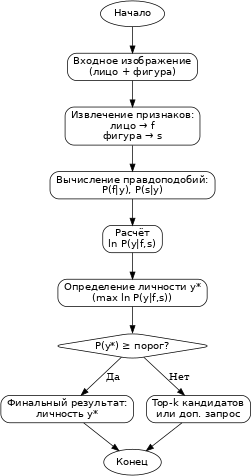
\includegraphics[width=0.6\textwidth,keepaspectratio]{images/3.png}
\caption{Частный случай ($K=2$): блок-схема предлагаемого алгоритма
байесовской реидентификации людей по~паре <<силуэт-лицо>>}
\label{fig:ch2/bayes-scheme}
\end{figure}

На~рис.~\ref{fig:ch2/bayes-scheme} представлена блок-схема
предлагаемого алгоритма для случая $K=2$. Сначала из~входного изображения с~помощью
двух нейросетевых моделей извлекаются вектора: $\mathbf{f}$~---
$d_f$-мерный вектор лица ($d_f=128$) и~$\mathbf{s}$~--- $d_s$-мерный вектор
силуэта (в~эксперименте $d_s=256$).

Затем эти признаки поступают в~модуль байесовского классификатора,
где вычисляются правдоподобия~(\ref{eq:ch2/gauss}) для каждого
из~$N=|Y|$ зарегистрированных в~системе личностей (классов идентификации).
Перемножая плотности (или суммируя лог-правдоподобия) согласно
формуле~(\ref{eq:ch2/bayes}), модуль выдает апостериорные вероятности
$P(y\mid\mathbf{f},\mathbf{s})$ по~всем классам $y=1,\ldots,N$.

Финальное решение~--- идентификатор~$y^*$~--- выбирается по~максимальной
апостериорной вероятности. Кроме того, вероятности могут быть
использованы для оценки уверенности: если максимум
$P(y^*\mid\mathbf{f},\mathbf{s})$ низок, система может воздержаться
от~однозначного ответа (выдать топ-$k$ кандидатов либо запросить
дополнительный образ). Ниже приведен алгоритм байесовской
идентификации.

\begin{longtable}{@{}p{0.97\textwidth}@{}}
\hline
\textbf{Алгоритм байесовской идентификации.}\\
\hline
\endfirsthead
\hline
\textbf{Алгоритм байесовской идентификации} (продолжение):\\
\hline
\endhead
\hline
\endfoot
\textbf{Вход:} изображение с~лицом и~фигурой человека.\\
\textbf{Шаг 1. Извлечение признаков:}\\
~~$\mathbf{f}:=\text{Embedder}_{\text{face}}(\text{изображение лица})$;\\
~~$\mathbf{s}:=\text{Embedder}_{\text{body}}(\text{изображение тела})$.\\
\textbf{Шаг 2. Байесовский классификатор:}\\
~~Для каждого $y\in Y$:\\
~~~~$p_f(y):=P(\mathbf{f}\mid y)$ по~формуле~(\ref{eq:ch2/gauss});\\
~~~~$p_s(y):=P(\mathbf{s}\mid y)$;\\
~~~~$p(y):=p_f(y)\cdot p_s(y)$ (так как $P(y)=\mathrm{const}$);\\
~~конец.\\
\textbf{Шаг 3. Идентификация:}\\
~~$y^*:=\arg\max_{y\in Y} p(y)$;\\
~~вывести $y^*$ как опознанную личность;\\
~~при необходимости вывести $p(y^*)$ как степень уверенности.\\
\end{longtable}

\subsection{Архитектура кодировщиков}\label{sec:ch2/encoders}

На~рис.~\ref{fig:ch2/vit} представлена архитектура Vision Transformer
для извлечения признаков изображения. Входное изображение делится
на~патчи фиксированного размера, которые подаются в~трансформерный
кодировщик. На~выходе используется классификационный токен ([CLS]) как
вектор изображения. MLP-голова отбрасывается~\cite{Dosovitskiy2020vit}.

В~предлагаемом подходе применяются две нейросетевые модели
(кодировщика), извлекающие векторные признаки из~изображений: одна~---
для лица, другая~--- для силуэта человека. Обе модели построены
на~базе Vision Transformer (ViT) и~используют функцию потерь
ArcFace~\cite{Deng2019arcface}, доказавшую свою эффективность для
задач биометрической идентификации.

\begin{figure}[htbp]
\centering
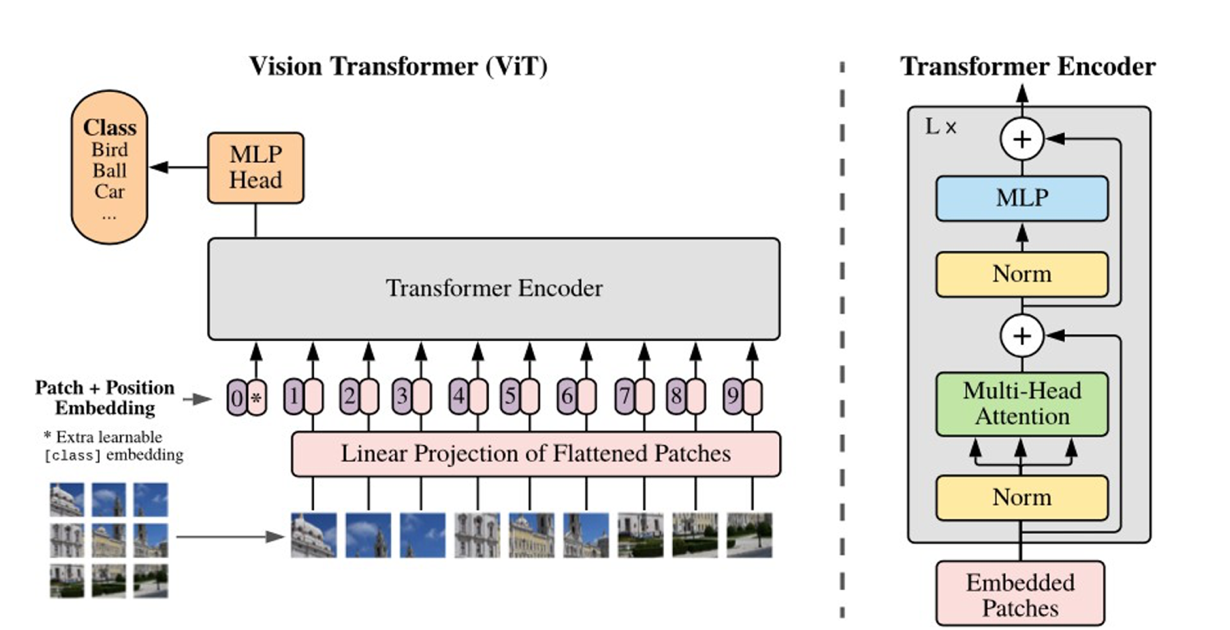
\includegraphics[width=0.85\textwidth,keepaspectratio]{images/2_2.png}
\caption{Архитектура Vision Transformer}
\label{fig:ch2/vit}
\end{figure}

Выбор архитектур эмбеддеров лиц и~силуэтов выполнялся не~эвристически,
а~на~основе совокупности критериев, учитывающих специфику задачи
реидентификации. В~качестве базовых рассматривались три класса
моделей:
\begin{itemize}
    \item классические сверточные сети (ResNet, IR-SE, EfficientNet,
          GhostNet);
    \item облегченные архитектуры, ориентированные на~работу
          в~условиях жестких ресурсных ограничений;
    \item трансформерные архитектуры типа Vision Transformer
          (ViT)~\cite{Dosovitskiy2020vit} с~механизмами самовнимания.
\end{itemize}

Критериями отбора служили:
\begin{itemize}
    \item дискриминативность признакового пространства (качество
          по~mAP, CMC/Rank-k на~репрезентативных наборах данных);
    \item устойчивость к~вариациям условий съемки (ракурс, освещение,
          частичная окклюзия);
    \item вычислительная сложность (количество параметров модели,
          объем операций на~одно изображение, задержка на~целевой
          аппаратной платформе);
    \item простота дообучения и~переноса на~новые домены при
          ограниченном числе размеченных примеров.
\end{itemize}

Предварительный анализ литературы~\cite{Deng2019arcface,Dosovitskiy2020vit,Hermans2017triplet}
и~пробные эксперименты показали, что модели на~основе ViT
в~сочетании с~угловыми функциями потерь типа
ArcFace~\cite{Deng2019arcface} формируют более компактные и~хорошо
разделимые кластеры эмбеддингов по~сравнению с~классическими
сверточными архитектурами при сопоставимой вычислительной нагрузке.
Это особенно выражено в~условиях значительной вариативности позы
и~освещения, характерных для задач реидентификации. При этом для
силуэтов требовалось более высокое разрешение глобальных контекстных
связей, чем могут обеспечить локальные свертки фиксированного размера.

С~учетом указанных обстоятельств в~качестве базовых эмбеддеров для
обеих модальностей выбраны архитектуры на~основе Vision Transformer
с~$L_2$-нормированием выходных векторов и~функцией потерь ArcFace.
Такой выбор обеспечивает баланс между дискриминативностью признаков,
устойчивостью к~внешним возмущениям и~возможностью практического
развертывания в~системах, работающих вблизи реального времени.

Детальное рассмотрение архитектуры Vision Transformer принципиально
важно в~контексте решаемой задачи, поскольку именно способ построения
токенов и~организация механизма самовнимания определяют геометрию
признакового пространства, в~котором далее реализуется байесовский
вывод. В~отличие от~классических сверточных сетей, ограниченных
локальным полем зрения и~жесткой иерархией уровней признаков, ViT
изначально оперирует последовательностью патч-токенов и~моделирует
глобальные зависимости между всеми фрагментами изображения. Это
обеспечивает следующие возможности кодировщика:
\begin{itemize}
    \item учитывать взаиморасположение ключевых областей (лицо, плечи,
          торс, нижняя часть силуэта) при формировании единого
          эмбеддинга;
    \item естественным образом интегрировать информацию о~фоне
          и~контексте сцены, что важно для устойчивости к~частичным
          окклюзиям и~пересечению траекторий;
    \item реализовывать инвариантность к~масштабным и~геометрическим
          преобразованиям за~счет позиционных кодировок
          и~многоуровневого внимания.
\end{itemize}

С~точки зрения реидентификации это означает, что вектор признаков
$\mathbf{f}$ или $\mathbf{s}$, извлекаемый ViT, отражает не~только
локальные текстурные особенности (рисунок одежды, черты лица),
но~и~конфигурацию тела в~целом. Такая глобальная репрезентация
существенно улучшает разделимость классов в~условиях изменяющихся поз
и~ракурсов, что подтверждается визуализациями t-SNE и~высокими
значениями mAP, полученными в~экспериментальной части работы. Кроме
того, использование единой архитектурной парадигмы для лица и~силуэта
упрощает последующую вероятностную интеграцию модальностей, так как
обе последовательности признаков подчиняются сходным статистическим
предпосылкам.

Для каждого изображения соответствующая модель извлекает вектор:
\begin{equation}\label{eq:ch2/embed}
    \mathbf{f}\in\mathbb{R}^{d_f},\quad \mathbf{s}\in\mathbb{R}^{d_s},
\end{equation}
где $\mathbf{f}$~--- вектор лица, $\mathbf{s}$~--- вектор силуэта.

Данная архитектура разбивает изображение на~непересекающиеся патчи,
кодирует их в~линейном пространстве и~передает в~стек
блоков самовнимания трансформера. На~выходе берется вектор [CLS]
как обобщенное представление всего изображения. Такая структура
эффективна как для лиц, так и~для тел и~служит универсальной
основой для обеих модальностей.

Функция потерь ArcFace~\cite{Deng2019arcface} применяется для
повышения дискриминативности представлений, вводя аддитивную угловую
поправку в~классификационную границу. Это обеспечивает формирование
векторов в~плотные и~разделенные кластеры. Альтернативно в~задачах
реидентификации может применяться Triplet
Loss~\cite{Hermans2017triplet}~--- метрическая функция, минимизирующая
расстояние между положительными парами и~увеличивающая расстояние
до~отрицательных. Однако в~проведенных в~работе экспериментах ArcFace
показал лучшую сходимость и~стабильность обучения.

Перед оцениванием параметров распределений и~вычислением плотностей вектора нормализуются по~$L_2$-норме:
\begin{equation}\label{eq:ch2/l2norm}
    \hat{\mathbf{f}}=\frac{\mathbf{f}}{\lVert\mathbf{f}\rVert_2},\quad \hat{\mathbf{s}}=\frac{\mathbf{s}}{\lVert\mathbf{s}\rVert_2}.
\end{equation}

В~отличие от~классического подхода центрирование признаков
относительно среднего по~обучающей выборке не~производится, поскольку
параметры многомерного нормального распределения (среднее
и~ковариационная матрица) для каждого класса оцениваются напрямую
по~обучающим данным.

Для объединения информации от~разных компонентов структуры
(в~рассматриваемом случае~--- разных модальностей, лица и~силуэта)
применяется байесовская схема. Итоговая логарифмическая апостериорная
вероятность принадлежности к~классу вычисляется как сумма логарифмов
модальности-зависимых плотностей:
\begin{equation}\label{eq:ch2/log-posterior}
    \log P(y\mid\hat{\mathbf{f}},\hat{\mathbf{s}})\propto\log P(\hat{\mathbf{f}}\mid y)+\log P(\hat{\mathbf{s}}\mid y).
\end{equation}

При этом весовые коэффициенты не~используются, то~есть вклад каждой
модальности считается равным. Эксперименты показали, что даже при
равномерной агрегации признаки обеих модальностей вносят значимый
вклад в~классификацию, а~предварительная $L_2$-нормализация
обеспечивает стабильную работу подхода вне зависимости от~размерности
векторов.

Одним из~важных преимуществ предложенного байесовского подхода
является его низкая вычислительная сложность и~хорошая
масштабируемость. В~отличие от~сложных методов с~обучаемыми
коэффициентами или методов на~основе глубоких сетей с~перекрестным
вниманием, предложенная модель требует лишь расчета махаланобисовых
(в~частном случае~--- евклидовых) расстояний до~центроидов классов
в~низкоразмерных пространствах
признаков, что реализуется эффективно даже для больших баз
идентифицируемых личностей. При увеличении количества личностей
(классов) вычислительная нагрузка растет линейно, обеспечивая легкое
масштабирование решения. Кроме того, подход обеспечивает простое
добавление новых модальностей и~адаптацию системы под изменения
условий съемки без необходимости переобучения сложных глубоких
архитектур.

В~отличие от~известных подходов к~задачам реидентификации человека,
в~которых, как правило, используется либо одиночная модальность
(силуэт или лицо), либо простое линейное объединение
признаков~\cite{Khachumov2015face,Koo2018multimodal,Vezzani2013reidsurvey},
разработанный в~работе метод опирается на~следующие принципиальные
положения.

\textit{Специализация кодировщиков под модальности.} Для лиц
и~силуэтов используются два отдельных кодировщика на~основе ViT,
каждый из~которых обучается с~учетом специфики соответствующей
модальности и~функции потерь ArcFace. Это обеспечивает формирование
эмбеддингов с~различной <<геометрией>> кластеров (меньший разброс для
лиц, больший~--- для силуэтов), что далее явным образом учитывается
в~байесовской модели.

\textit{Нормировка и~согласование признаковых пространств.}
Применение $L_2$-нормировки~(\ref{eq:ch2/l2norm}) приводит эмбеддинги
к~единичной сфере, обеспечивая сопоставимость расстояний
и~корректность предположения о~многомерной нормальности распределений
внутри классов. Это создает основу для строгой вероятностной
интерпретации, в~то~время как во~многих работах объединение признаков
носит сугубо эвристический характер.

\textit{Вероятностная интеграция вместо фиксированных весов.} Вместо
жестко заданного веса~$\alpha$ при объединении признаков лица
и~силуэта, как это часто делается в~линейных схемах, в~работе
используется байесовская модель~(\ref{eq:ch2/bayes})-(\ref{eq:ch2/gauss}),
в~которой вклад модальностей задается через их правдоподобия. Таким
образом, модальность с~более устойчивым и~узким распределением
(например, лицо при хороших условиях съемки) автоматически оказывает
больший вклад в~апостериорную вероятность, тогда как <<шумная>>
модальность (размытый силуэт, сильная окклюзия) в~меньшей степени
влияет на~итоговое решение.

\textit{Возможность работы при отсутствии одной из~модальностей.}
Благодаря вероятностной постановке при отсутствии лицевого или
силуэтного канала классификатор может быть естественным образом
приведен к~учету только оставшейся модальности, что формально
соответствует маргинализации по~отсутствующему наблюдению. Это
отличие принципиально от~методов, использующих жесткое слияние
векторов фиксированной размерности.

Совокупность перечисленных принципов обеспечивает превосходство
разработанного подхода над существующими решениями в~аспектах
устойчивости к~отсутствию или деградации отдельной модальности,
интерпретируемости принимаемых решений и~соответствия статистическим
предпосылкам, лежащим в~основе байесовского вывода. Результаты
сравнительного анализа по~метрике mAP на~наборах данных CUHK03,
Market-1501 и~MARS (см.~раздел~3.3) подтверждают, что такая схема
интеграции признаков обеспечивает уровень качества, сопоставимый или
превосходящий передовые методы при сопоставимой вычислительной
сложности.

Одним из~ограничений предложенного подхода является использование
предположения о~нормальности распределения признаков в~каждой
модальности, что может не~всегда идеально соответствовать реальным
данным, особенно при наличии выбросов или нетипичных наблюдений. Для
преодоления этого ограничения рекомендуется в~дальнейшем рассмотреть
применение более гибких статистических моделей, в~частности смесей
гауссовых распределений или непараметрических методов оценки
плотностей. Также можно рассмотреть устойчивость модели к~шумам
и~искажениям в~данных и~возможности ее улучшения через использование
робастных статистических методов или предварительной фильтрации
входных данных.

Дальнейшие направления работы связаны с~расширением модели
несколькими биометрическими модальностями и~внедрением более гибких
ковариационных структур, обеспечивающих учет попарной зависимости
признаков. Также перспективно исследовать онлайн-обучение параметров
распределений для поддержки динамических баз персоналий и~адаптацию
порога уверенности под изменяющиеся условия съемки.

\section{Выводы по~главе}\label{sec:ch2/conclusion}

Во~второй главе изложен комплексный подход к~распознаванию
многокомпонентной структуры по~ее разрозненным частям, развернутый
на~наиболее представительном частном случае~--- распознавании
и~реидентификации человека по~паре <<силуэт-лицо>> ($K=2$),~--- основанный
на~современных алгоритмах
компьютерного зрения и~методах глубокого обучения. Важнейшим этапом
становится детектирование компонентов структуры (в~рассматриваемом
случае~--- силуэтов и~лиц), для чего предложено
использовать модель YOLOv8, обладающую высокой скоростью обработки
и~точностью определения объектов. Модификация стандартной функции
потерь, учитывающая специфику обнаружения вложенного компонента
внутри внешнего (в~частном случае~--- лиц внутри силуэтов),
обеспечивает более точный поиск ключевых областей на~изображении,
особенно в~сложных и~динамичных сценах. Это снижает количество ложных
срабатываний и~повышает надежность идентификации даже при наличии
частичных перекрытий или нетривиальных условий освещения.

Следующим существенным шагом является формирование эмбеддингов, то~есть
числовых векторных представлений лиц и~силуэтов. Внимание уделено
разнообразным архитектурам~--- от~классических сверточных сетей
(ResNet, IR-SE, GhostNet, EfficientNet) до~Vision Transformer (ViT).
Выбор ViT обоснован ее способностью улавливать глобальные контекстные
взаимосвязи на~изображении, что особенно важно при анализе
неоднородных входных данных. Наличие гибких механизмов внимания
и~возможность масштабирования делают ViT перспективным инструментом
для формирования информативных эмбеддингов в~задачах реидентификации.

Основой методики стало объединение (комбинирование)
эмбеддингов компонентов структуры (в~рассматриваемом случае~--- лиц
и~силуэтов) с~использованием байесовской вероятностной
модели и~MAP-критерия. Подобная стратегия обеспечивает более полное
описание распознаваемой структуры и~повышает точность распознавания. Адаптивный вклад
каждой модальности достигается через ковариационные матрицы класса
в~гауссовых правдоподобиях, что устраняет необходимость в~ручной
настройке весовых коэффициентов и~обеспечивает корректное поведение
решающего правила при временном отсутствии или зашумлении одной из~модальностей.

В~заключительной части главы рассмотрены вопросы разработки
комбинированной метрики для идентификации, подтверждены
детерминированность и~массовость предложенного алгоритма. Решающее
правило MAP представляет собой прямое (неитеративное) вычисление
максимума апостериорной вероятности и~завершается за~конечное число
операций. Детерминированность обеспечивается строго заданными
исходными данными, а~массовость~--- возможностью масштабировать
вычисления на~любые объемы данных при сохранении корректного
функционирования алгоритма. Таким образом, глава демонстрирует
комплексный подход к~распознаванию многокомпонентной структуры
по~ее частям, совмещающий передовые средства детектирования,
формирования эмбеддингов и~метрики идентификации; в~рассматриваемом
частном случае ($K=2$) подход открывает
перспективы для высокоточных систем распознавания и~реидентификации
человека.

В~ходе разработки частных методик и~алгоритмов возник ряд проблем,
обусловленных как характеристиками исходных данных, так
и~ограничениями целевой эксплуатационной среды
информационно-поисковой системы. Ниже последовательно изложены
ключевые трудности и~примененные решения в~контексте детектирования,
формирования признаковых представлений и~настройки гиперпараметров
комбинированной метрики с~последующей интеграцией модальностей.

На~этапе детектирования основными источниками ошибок стали сложные
сцены с~высокой плотностью объектов, вариативным освещением
и~частичными перекрытиями, а~также случаи, когда лицо присутствует
как <<вложенная>> область внутри силуэта и~фиксируется под
нестандартными ракурсами. Это приводило к~каскадному эффекту:
ошибочная локализация формировала некорректные входные данные для
дальнейших этапов. Для снижения влияния указанных факторов усилена
часть, отвечающая за~качество локализации: проведена донастройка
детектора на~доменно близких выборках с~акцентом на~<<трудные>>
примеры (окклюзии, слабое освещение), модифицирована функция потерь
с~увеличением веса ошибок по~мелким лицевым областям и~введены
дополнительные проверки согласованности между маской силуэта
и~найденным лицом. Дополнительно применены процедуры калибровки
порогов постобработки (NMS/score-threshold) и~адаптивной фильтрации
по~контекстным признакам сцены, что снизило количество пропусков
и~ложных срабатываний без существенного роста вычислительных затрат.

При построении признаковых представлений для лица и~силуэта выявлены
два класса проблем: (1)~падение дискриминативности при сильной
вариативности ракурса и~позы; (2)~переобучение на~ограниченных
фрагментах данных. Для решения первой проблемы применены архитектурные
и~процедурные меры: нормализация входов, усиленные аугментации
(в~том~числе имитация освещенности/окклюзий), а~также согласование
размеров и~центров обрезки с~характерными зонами
информативности для каждой модальности. Для борьбы с~переобучением
использованы регуляризация с~контролем нормы весов и~признаков,
сглаживание меток для стабилизации градиентов, а~при обучении метрик~---
комбинации Triplet/ArcFace-подобных потерь, обеспечивающие разнесение
межклассовых расстояний при контролируемой компактности
внутриклассовых кластеров. На~валидации проводился контроль
по~интегральным метрикам (mAP, CMC/Rank-k) и~анализу распределений
оценок, что позволило своевременно выявлять деградацию обобщающей
способности.

Существенные трудности возникали при выборе весов для объединения
признаков компонентов структуры (в~рассматриваемом случае~--- лицевых
и~силуэтных признаков): фиксированные коэффициенты
демонстрировали нестабильность при смене сцены и~условий съемки.
Для снятия этой проблемы разработан алгоритм автоматической настройки
ключевого гиперпараметра комбинированной метрики, учитывающий
показатели качества детектирования и~локальные признаки надежности
модальности. Использована вероятностная (байесовская) схема
интеграции, в~которой вклад модальностей масштабируется их текущей
достоверностью: при уверенной локализации лица возрастает вес
лицевого признакового вектора, при частичной видимости~--- приоритет
смещается в~сторону силуэта. Такой подход обеспечил адаптацию решения
к~контексту кадра без ручной подстройки и~рост итоговых показателей
при сопоставимой вычислительной сложности.

В~рамках требований близкой к~реальному времени обработки выявлена
проблема избыточной задержки при использовании тяжелых конфигураций
детектора и~эмбеддера. Для ее разрешения выполнено профилирование
конвейера с~последующей оптимизацией узких мест: упорядочивание
вычислений с~уменьшением межэтапных копирований, квантизация
некоторых промежуточных представлений, а~также ограничение числа
кандидатов после детектирования на~основе доверия и~геометрии.
Пороговые значения решений согласованы с~эксплуатационными метриками
(ROC/PR-анализ, оптимизация по~F-мере в~зоне интереса), что
обеспечило баланс между точностью и~временем отклика.

Отмеченные шумы разметки и~дисбаланс классов осложняли объективную
оценку качества. Для их компенсации проведены очистка
и~стратифицированные выборки, а~также перекрестная валидация
с~отчетными доверительными интервалами для ключевых метрик.
Единообразные протоколы предобработки, фиксированные генераторы
случайных чисел и~сохранение контрольных конфигураций обеспечили
воспроизводимость результатов и~сопоставимость с~базовыми методами.

В~совокупности изложенные меры устранили критичные узкие места
контура и~обеспечили согласованную работу компонентов: детектор
формирует корректные входы, эмбеддинги сохраняют дискриминативность
в~сложных условиях, а~адаптивная интеграция модальностей повышает
устойчивость итогового решения без выхода за~рамки допустимых
вычислительных затрат. Полученные эффекты подтверждаются ростом
интегральных показателей качества на~репрезентативных наборах данных
при соблюдении требований к~задержке и~стабильности.
